\chapter{Result and Analysis}
	To evaluate the performance of our various algorithm implementations, we use Python's \texttt{timeit} module to measure the execution time of both the standard \texttt{NetworkX.shortest\_path()} function and our custom algorithm. The following code demonstrates our approach:
	
	\begin{lstlisting}
		timer = timeit.Timer(lambda: nx.shortest_path(G, start_node, end_node))
		nx_time = min(timer.repeat(5, 100))
		print("NetworkX time:", nx_time)
		
		timer = timeit.Timer(lambda: algorithm(G, start_node, end_node, preprocessor))
		algo_time = min(timer.repeat(5, 100))
		print("Algorithm time:", algo_time)
		
		print(f"NetworkX's algorithm takes {nx_time / algo_time:.4%} of Algorithm's time")
	\end{lstlisting}
	
	This code operates as follows:
	\begin{enumerate}
		\item \textbf{Timing Setup:}  
		\begin{itemize}
			\item We create a \texttt{Timer} object from the \texttt{timeit} module with a lambda function that calls either \texttt{nx.shortest\_path(G, start\_node, end\_node)} or our custom \texttt{algorithm(G, start\_node, end\_node, preprocessor)}.
		\end{itemize}
		\item \textbf{Repeating the Measurement:}  
		\begin{itemize}
			\item The method \texttt{repeat(5, 100)} executes the lambda 100 times per iteration, repeated over 5 iterations. This returns a list of execution times.
		\end{itemize}
		\item \textbf{Selecting the Best Time:}  
		\begin{itemize}
			\item Instead of averaging the results, we use \texttt{min()} to select the lowest execution time. This minimum value represents a lower bound of the runtime under optimal conditions. Variability due to system load or background processes typically results in higher values, so using the minimum helps mitigate these effects.
		\end{itemize}
		\item \textbf{Performance Comparison:}  
		\begin{itemize}
			\item Finally, we compare the performance by printing the ratio of \texttt{nx\_time} to \texttt{algo\_time}. This ratio indicates how much faster (or slower) our custom algorithm is relative to NetworkX's implementation.
		\end{itemize}
	\end{enumerate}
	
	By timing both the standard and custom implementations in this way, we ensure a system-independent baseline for performance, making it possible to assess the inherent efficiency of our algorithm.

	 \section{Version 1: Basic Dijkstra's Algorithm}
	 	Running the timing code on this version produced the following output:
	 	\begin{verbatim}
	 		NetworkX time:  0.6769123002886772
	 		Algorithm time:  21.229514400009066
	 		NetworkX's algorithm takes 3.1885% of Algorithm's time
	 	\end{verbatim}
	 	While not optimal, this version serves as a valuable baseline for comparing subsequent, more advanced versions.

	 \section{Version 2: A* Search Algorithm}
	 	Running the timing code on this version produced the following output:
	 	\begin{verbatim}
			NetworkX time:  0.7038580998778343
			Algorithm time:  19.783792700152844
			NetworkX's algorithm takes 3.5578% of Algorithm's time
	 	\end{verbatim}
	 	
	 	This represents a \(\frac{3.5578}{3.1885} \approx 1.11\times\) improvement in execution time compared to Version 1. \newline
	 	
	 	Such a performance gain is consistent with the theoretical benefits of the A* algorithm, where a simple heuristic helps prioritize the exploration of nearer edges. As the size of the graph increases, we expect this improvement to become even more pronounced.
	 
	 \section{Version 3: Bidirectional Dijkstra's Algorithm}
	 	Running the timing code on this version produced the following output:
	 	\begin{verbatim}
	 		NetworkX time:  0.6851798999123275
	 		Algorithm time:  16.339504099916667
	 		NetworkX's algorithm takes 4.1934% of Algorithm's time
	 	\end{verbatim}
	 
		 This represents a \(\frac{4.1934}{3.5578} \approx 1.18\times\) improvement over Version 2. 
		 
		 \begin{figure}[H]
		 	\centering
		 	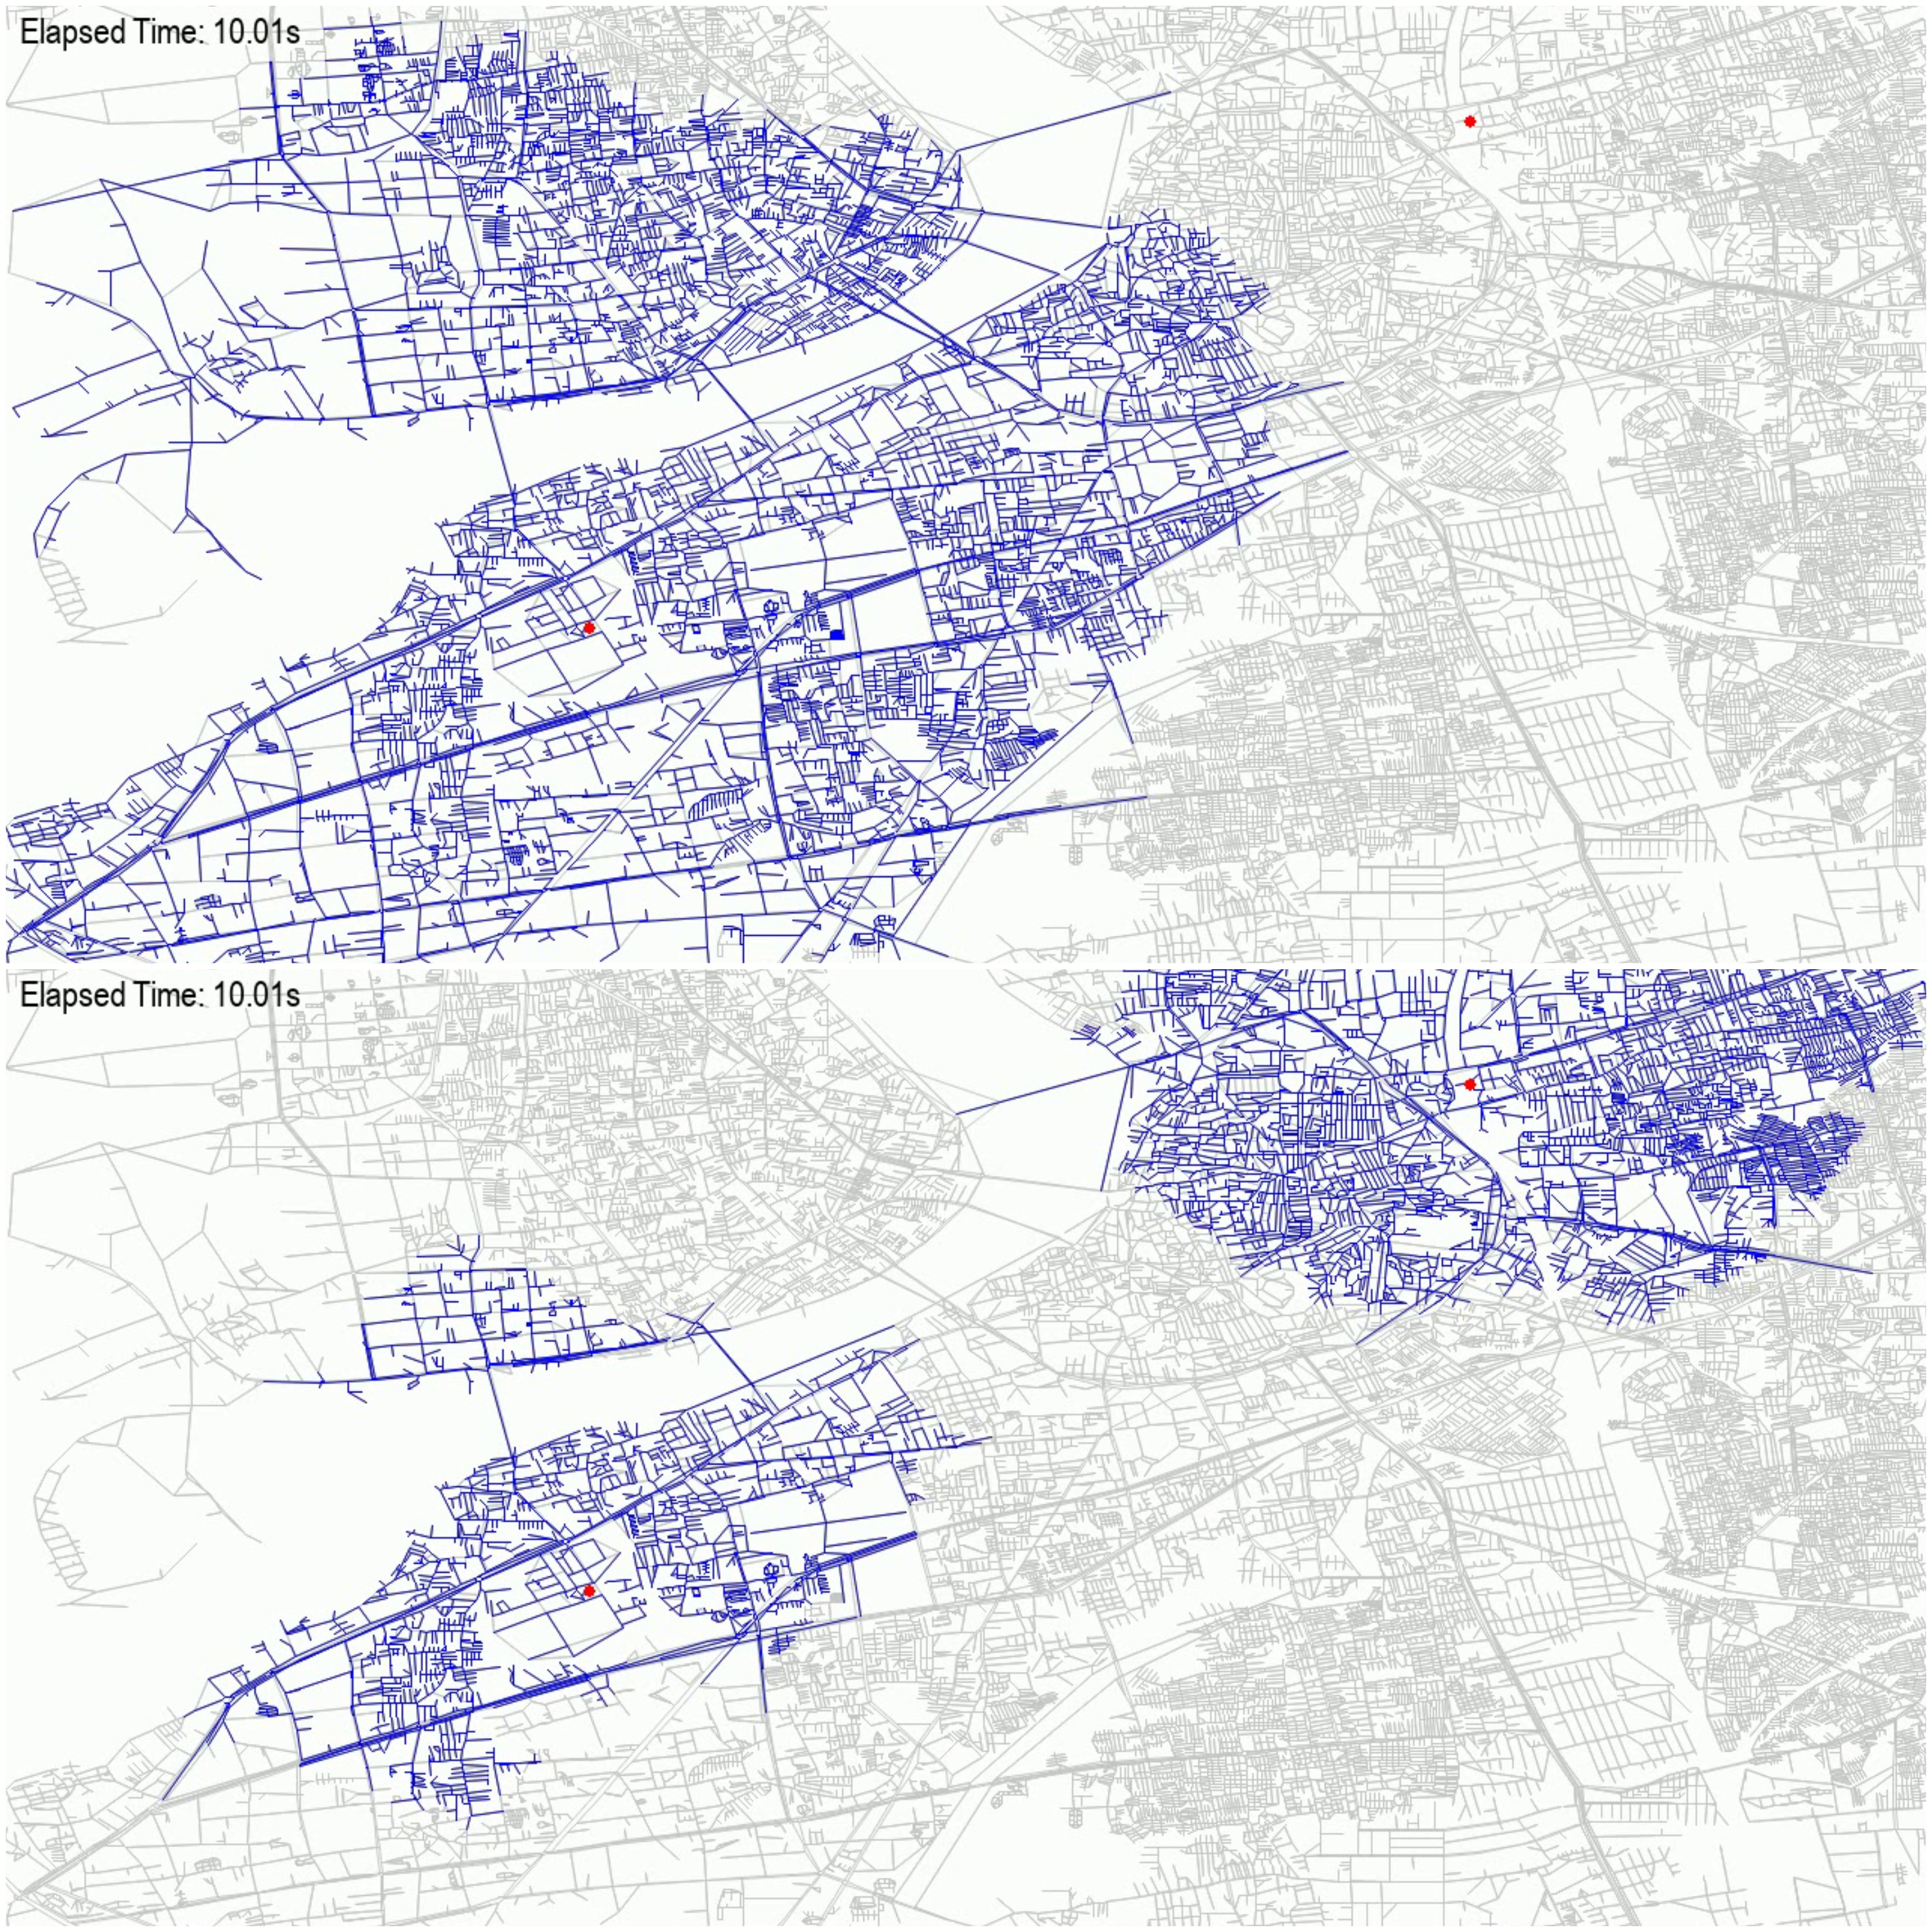
\includegraphics[width=0.7\textwidth]{astar_vs_bidijkstra.png}
		 	\caption{Visualization of explored edges at $t$ $=$ $10s$ for Version 2 (A* search) vs Version 3 (Bidirectional Dijkstra's).}
		 	\label{fig:bidirectional_dijkstra_vs_astar}
		 \end{figure}

		 While this version employs a less sophisticated path exploration strategy compared to the previous one, it achieves enhanced performance because bidirectional Dijkstra's algorithm can terminate as soon as the forward and backward searches meet. In contrast, A* continues until the target node is fully expanded, making its performance heavily dependent on the quality of the heuristic used.
	 
	 \section{Version 4: Bidirectional A* Search Algorithm}
	 	Running the timing code on this version produced the following output:
	 	\begin{verbatim}
	 		NetworkX time:  0.7203088998794556
	 		Algorithm time:  13.28147240029648
	 		NetworkX's algorithm takes 5.4234% of Algorithm's time
	 	\end{verbatim}
	 	
	 	This represents a \(\frac{4.1934}{3.5578} \approx 1.18\times\) improvement over Version 3. \newline \vspace{4mm}
	 	
	 	The enhanced performance in this version stems from integrating the strengths of the previous two: employing a heuristic to guide path exploration and reducing the search space through bidirectional search.
	 
	 \section{Final Version: Bidirectional A* Search with ALT Preprocessing}
	 	Running the timing code on this version produced the following output:
	 	\begin{verbatim}
	 		NetworkX time:  0.6841806997545063
	 		Algorithm time:  4.040331699885428
	 		NetworkX's algorithm takes 16.9338% of Algorithm's time
	 	\end{verbatim}
	 	
	 	This represents a \(\frac{5.4234}{16.9338} \approx 3.12\times\) improvement in execution time compared to Version 4. \vspace{4mm}
	 	
	 	The substantial performance enhancement in this version is due to the integration of bidirectional A* search with the ALT preprocessing technique. By precomputing distances to strategically chosen landmarks, the ALT method provides more accurate heuristic estimates, effectively reducing the search space during query execution.\vspace{4mm}
	 	
	 	Although the preprocessing phase requires a non-trivial amount of time, this upfront cost is amortized over numerous queries, resulting in significantly faster average query responses. This approach is particularly beneficial in large-scale road networks, where rapid query times are essential.
	 	
	 	\begin{figure}[H]
	 		\centering
	 		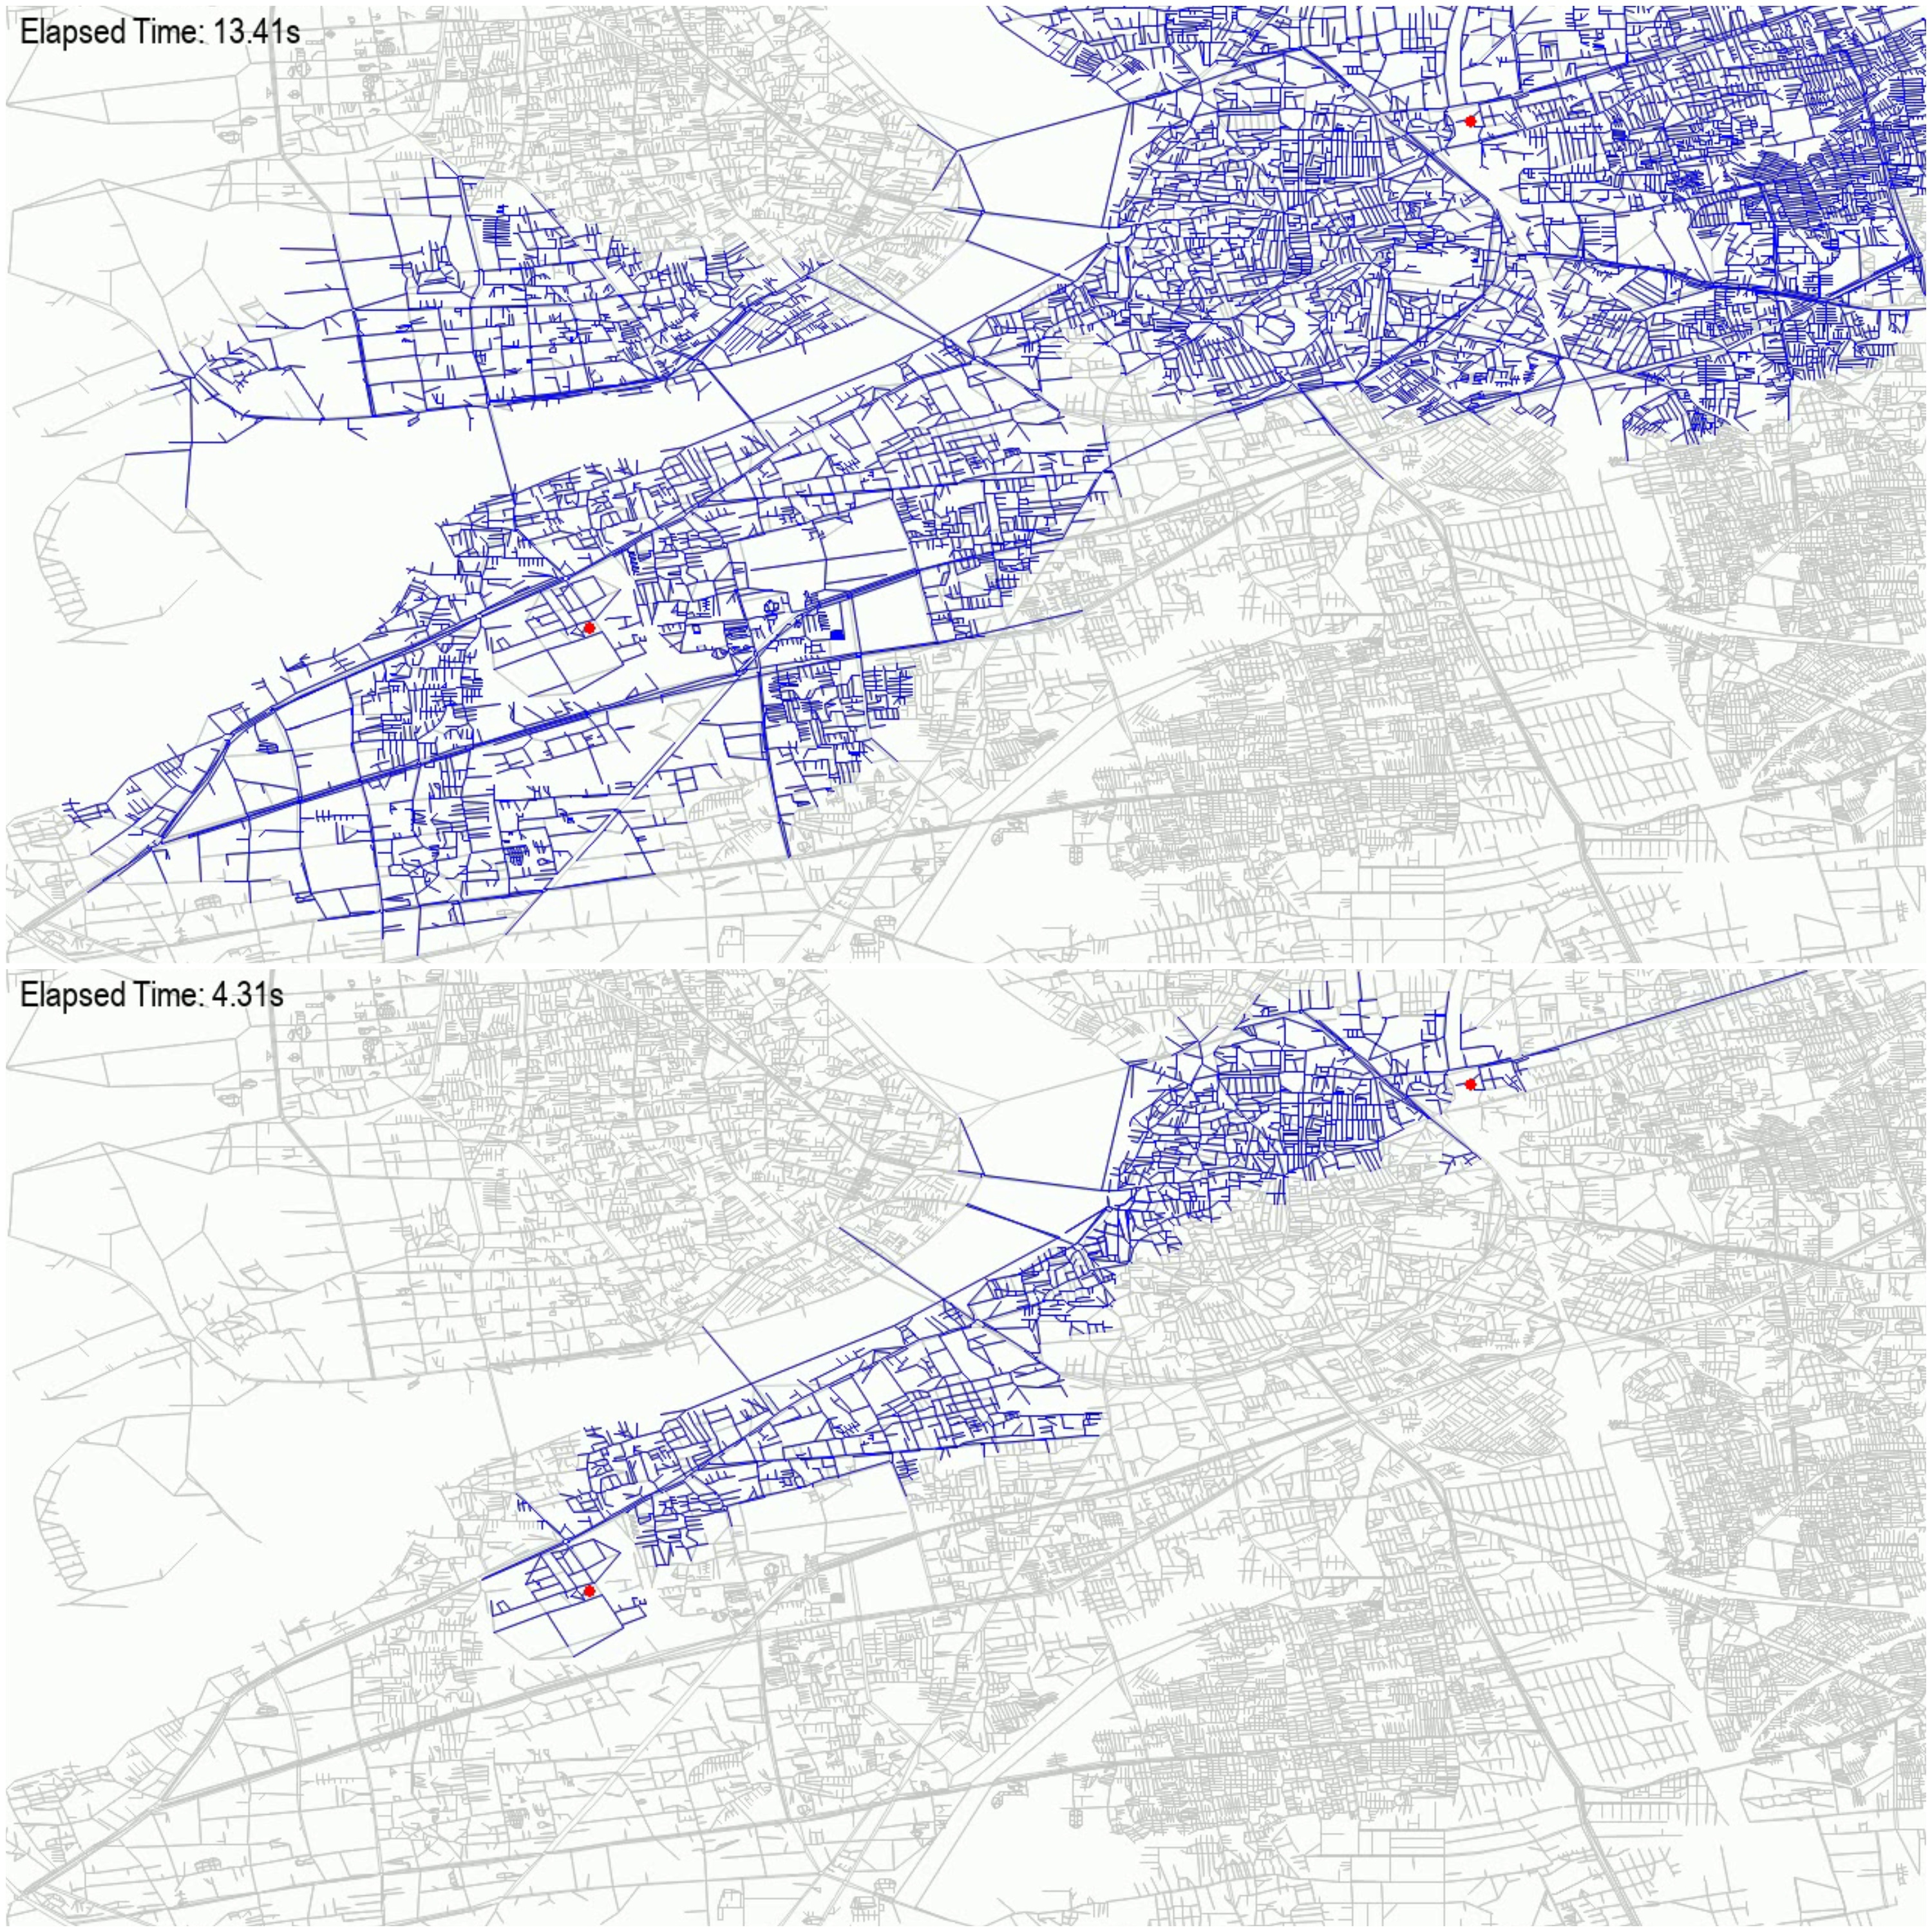
\includegraphics[width=0.7\textwidth]{final_vs_biastar.png}
	 		\caption{Visualization of all the explored edges in Version 4 (Bidirectional A*) vs Final Version (ALT + Bidirectional A*).}
	 		\label{fig:bidirectional_astar_vs_final}
	 	\end{figure}
	 	
	 	To get a more concrete comparison of the final version of our algorithm against NetworkX's we use the following code which compares their performances over multiple randomly selected source-destination pairs. The process is broken down into several steps:
	 		
	 		\begin{enumerate}
	 			\item \textbf{Generating random source-destination pairs} and storing them in a list:
	 			\begin{lstlisting}
	 				nodes_list = list(G.nodes)
	 				sources_dests = list()
	 				for i in range(0, 100):
	 				sources_dests.append( {"source": random.choice(nodes_list),
	 					"dest": random.choice(nodes_list)} )
	 			\end{lstlisting}
	 			
	 			\item \textbf{Preprocessing the graph}:
	 			\begin{lstlisting}
	 				preprocessor = ALTPreprocessor(G)
	 			\end{lstlisting}

	 			\item \textbf{Comparing execution times} using the scheme used previously, i.e. taking the minimum of a $100$ runs:
	 			\begin{lstlisting}
	 				def compare_times(graph, source, dest):
	 				timer = timeit.Timer(lambda: nx.shortest_path(graph, source, dest, weight='length'))
	 				nx_time = min(timer.repeat(5, 100))
	 				
	 				timer = timeit.Timer(lambda: bidirectional_alt_query(graph, source, dest, preprocessor))
	 				algo_time = min(timer.repeat(5, 100))
	 				
	 				return nx_time / algo_time * 100
	 			\end{lstlisting}
	 			
	 			\item \textbf{Aggregating results} by iterating over all the generated source-destination pairs and storing them in a list, and then taking the mean of these results:
	 			\begin{lstlisting}
	 				percentanges = list()
	 				for source_dest in sources_dests:
	 				try:
	 				percentanges.append(compare_times(G, source_dest["source"], source_dest["dest"]))
	 				except:
	 				nx.exception.NetworkXNoPath
	 				
	 				mean_percentage = sum(percentanges) / len(percentanges)
	 				print(f"NetworkX's algorithm takes {mean_percentage:.4f} of Algorithm's time")
	 			\end{lstlisting}
	 		\end{enumerate}
	 	Here is the output from this test:
	 	\begin{verbatim}
	 		NetworkX's algorithm takes 196.4728% of Algorithm's time
	 	\end{verbatim}
	 	Which means our algorithm is $\approx 2\times$ faster than NetworkX's \texttt{shortest\_path} implementation on average. This is expected because NetworkX uses Dijkstra's algorithm by default. In the 'SVNIT $\to$ Surat Railway Station' route, the benefits of preprocessing are minimal compared to a plain Dijkstra's search, making it an edge case for our enhancements.
	 